\chapter{Contiki Folder and Makefile Structure} \label{ApdxContiki}

\section{Folder structure of Contiki} \label{ApdxFolder}
When porting a new platform to Contiki, the three folders inside a Contiki distribution where additions need to be made are cpu, examples and platform. The content in these folders are as described below. The location of the Contiki distribution is represented by the path `CONIKI'. The port of nrf51822 \gls{soc} with its PCA10000 board also follows this convention.

\paragraph{CONTIKI/cpu}In this folder, all the files contain implementation which is solely dependent on the \gls{soc} is present. This includes the code for the processor abstraction, the drivers of the peripherals of the \gls{soc}, makefile with commands for compiling and linking the code, linker file and the documentation of these implementation. The boot-loader  or start-up code, if required is also present here. The peripheral drivers for peripherals such as timers and serial port must use the \gls{api} format of Contiki so that the libraries of Contiki using these peripherals can operate correctly. The exact implementations of these drivers is explained in section \ref{peripheralsContiki}. 

\paragraph{CONTIKI/platform} An \gls{soc} over time has increasing number of boards or systems that are based on it and these are referred as platforms in this folder. Every board has its own folder in this platform folder which contains files which contain implementation which is dependant on the particular board. These include the specification of the connections to the LEDs, buttons, sensors and serial ports, power sources, the clock sources, memories present and any other board specific details. Any peripheral driver implementation specific to the board is present here. The default project specifications such as the source and frequency of clock and serial baud-rate are defined here. The main function where the execution of the program starts and initialization of all the peripherals and libraries used by Contiki happens is present here.

\paragraph{CONTIKI/examples} The examples folder contains all the files related to projects that are implemented using Contiki with any of the supported hardware platforms. The makefile where the make command is executed is present here. The compiled object and binary files are also stored here. The default specifications of the platform can be overridden by creating a \texttt{project-conf.h} in the specific example.


\section{Makefile structure of Contiki} \label{ApdxMakefile}

\textbf{Introduction to makefile and include.}
There are multiple makefiles present across different folders that are included in the way shown in figure \ref{MakefileLevel} to form the complete makefile. In the most basic form these are the makefile in the example folder, `makefile.include' in the Contiki root folder, `makefile.TARGET' in the specific platform folder and `makefile.CPU' in the specific cpu folder, where TARGET and CPU are specific to the project. The port of Contiki to nrf51822's platform follows this convention too.

\begin{figure}[h]
\centering
\def\svgwidth{0.93\columnwidth}
\input{./Images/MakefileLevel.pdf_tex}
\vspace{-10pt}
\caption{Structure of Makefile inclusion in Contiki \gls{os} to form an example specific one}
\label{MakefileLevel}
\end{figure}

%Makefile where the project is present i.e. in the example folder
%-Makefile indicating the target platform (if not already specified)
%-Makefile.include in root CONTIKI directory
%--Makefile of applications, if any are required
%--Makefile of the target, present in the platform directory
%---Makefile of the \gls{soc}, present in the cpu directory

The makefile in the project specific example folder, the different project source files are specified and the `makefile.include' present in the root CONTIKI folder is added. `makefile.inlcude' glues together all the required components of Contiki and provides the default implementation of compiling and linking. The target makefile in the specific platform directory is included here. In `makefile.TARGET' the source files present in this directory are added, any Contiki modules required are added and the \gls{soc} or \gls{mcu} makefile in the specific directory is added. The \gls{soc} or \gls{mcu} makefile adds all the source files present in the CPU directory, specifies the command for compiling the code, linking the objects generated, uploading the executable binary or hex file.

The makefile in the example folder is where the make command is called. The operations that can be performed with this make command depends on the makefile. Usually the operations are cleaning (removing the object and binary files), compiling the source files into object files , linking these object files to create an executable file, creating a binary file from this executable file, uploading the binary to the \gls{soc} to start execution and so on. For the nrf51822 \gls{soc} additional operations of uploading the SoftDevice and erasing the flash are supported.



\chapter{Advertisement Logger's Implementation} \label{ApdxAdvLog}

\section{Scanning \texorpdfstring{\gls{ble}}{BLE} Advertisements}

According to the Bluetooth 4.0 Core specifications, an advertisement event consists of an advertising device periodically send advertisement packets. The interval of these advertising events can range from 20 ms to 10 s. In each of these advertising events an advertiser sends an advertising packet in each channel in an interval of 10 ms starting with channel 37. The objective of a BLE advertisement scanner would be to be able to receive the packets from at least one channel in an advertisement event, while saving power. To achieve this trade off, the radio duty cycles between receiving and disabled state, while being in the next advertising channel every time it is switched on. The total time of this periodic event is known as the \emph{Scan Interval}, while the time the radio is on is known as \emph{Scan Window}. The figure\footnote{\href{https://devzone.nordicsemi.com/question/2535/what-is-the-minimum-time-for-a-app-and-a-peripheral-to-create-a-connection/}{https://devzone.nordicsemi.com/question/2535/what-is-the-minimum-time-for-a-app-and-a-peripheral-to-create-a-connection/}} \ref{fig:AdvScanBLE} depicts this process.

\begin{figure}[h]
\centering
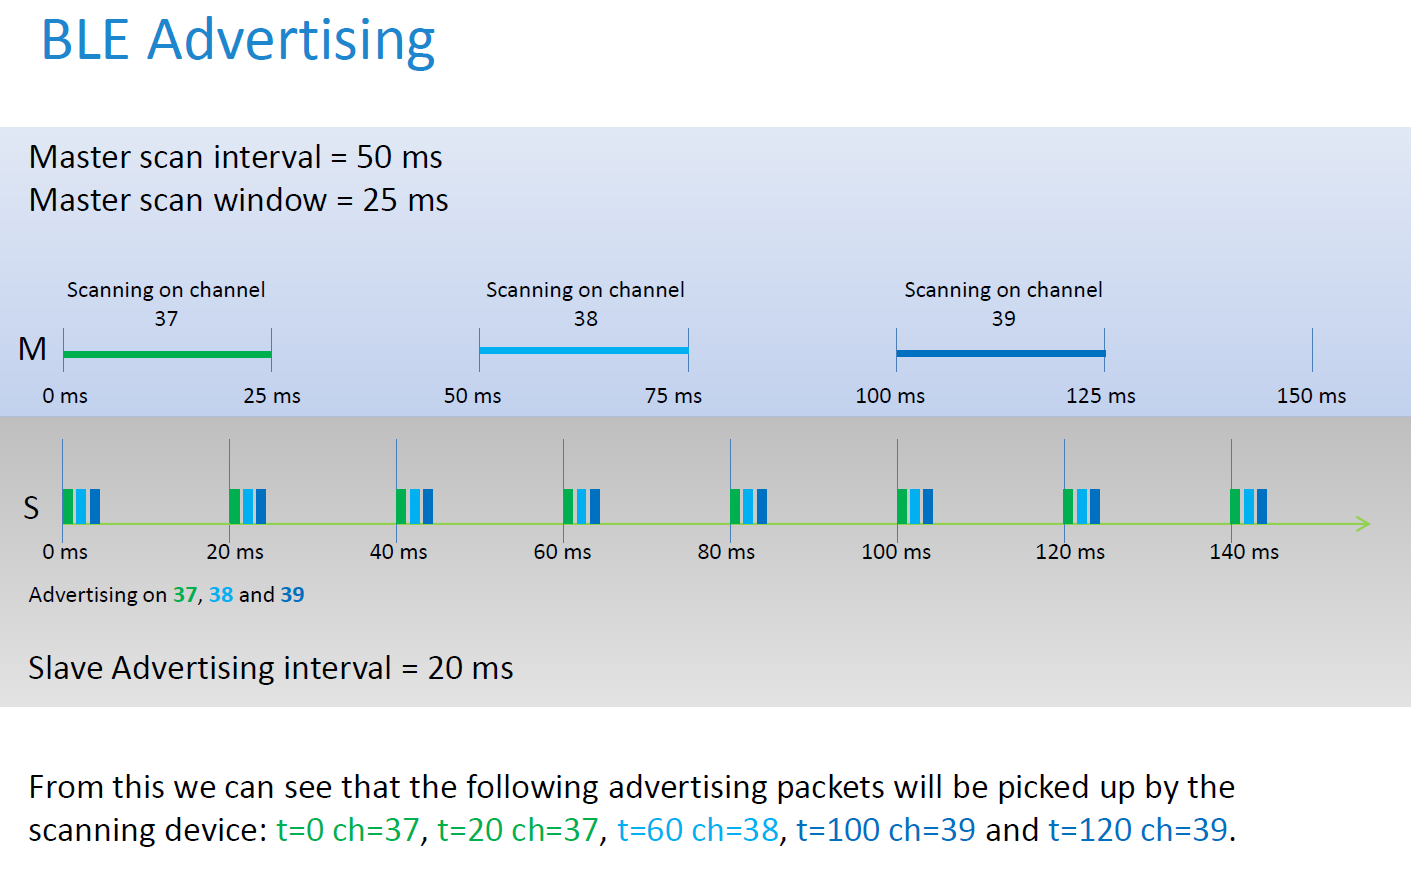
\includegraphics[width=\textwidth]{AdvScanBLE}
\caption{Scanning BLE advertisements}
\label{fig:AdvScanBLE}
\end{figure}

\section{Software Architecture}
The following flow charts explain the software architecture of the \emph{Advertisement Logger}.
\subsection{Main Function}
The execution of the program starts with the main function after reset as depicted by figure \ref{fig:main_chart}. Note that the radio is initialized to continuously receive packets once it has started while also measuring the received signal strength \acrshort{rssi}.
\begin{figure}[h]
\centering
\vspace{80pt}
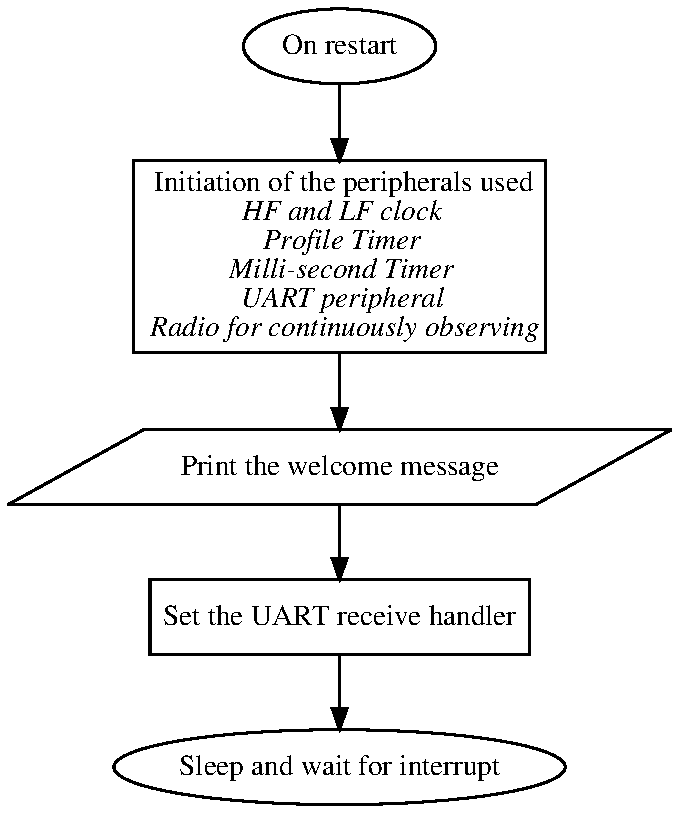
\includegraphics[scale=0.8]{main_chart}
\caption{Main function flowchart}
\vspace{80pt}
\label{fig:main_chart}
\end{figure}
\clearpage

\subsection{UART String Receive Handler}
The UART String Receive handler which gets a string sent to the \gls{soc} through an unsigned character pointer checks if the string is either \texttt{START} or \texttt{STOP} so that the scanning of the advertisements can be started or stopped respectively.
\begin{figure}[h]
\centering
\vspace{50pt}
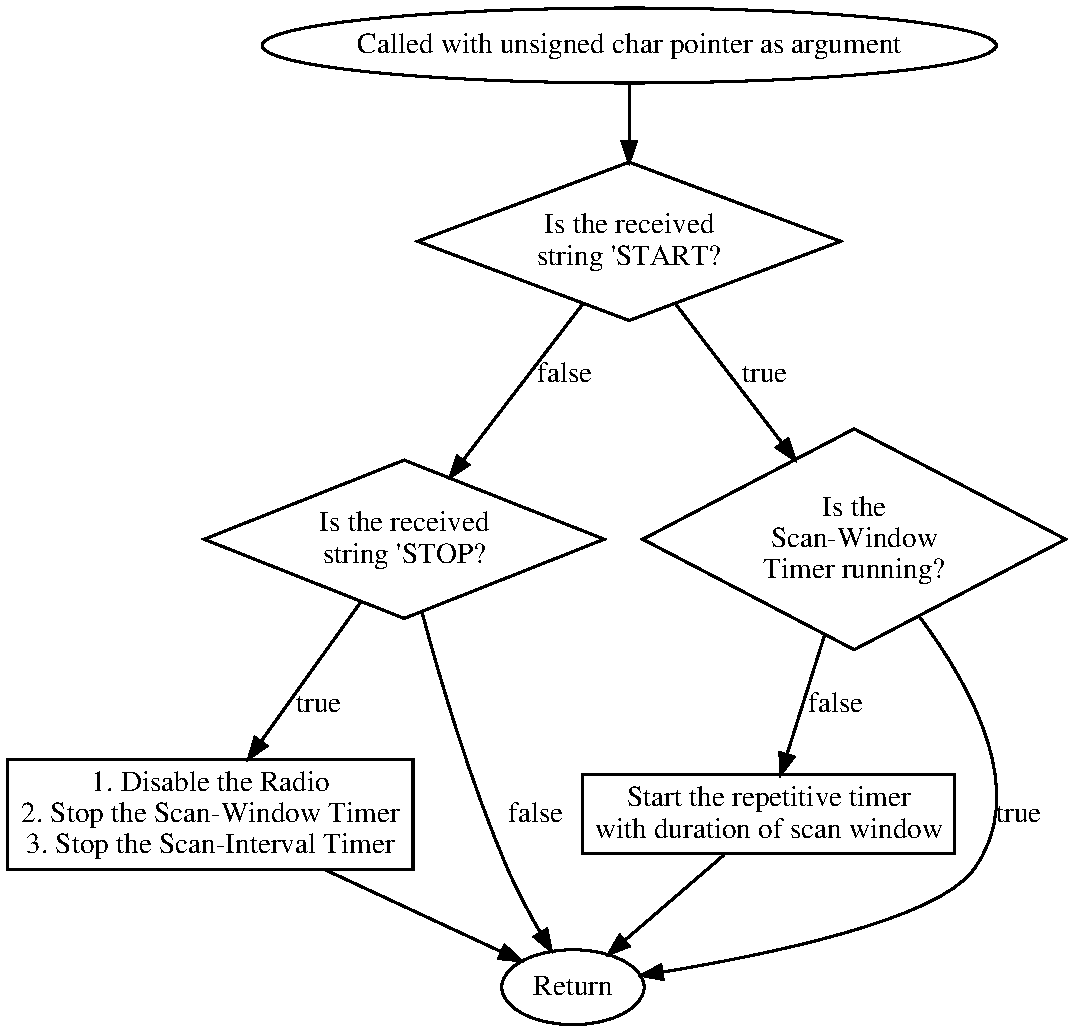
\includegraphics[scale=0.8]{UartISR_chart}
\caption{UART string receive handler flowchart}
\vspace{51pt}
\label{fig:UartISR_chart}
\end{figure}
\clearpage

\subsection{Scan Interval Timer Handler}
The scan interval timer is a repetitive timer with an interval equal to the scan interval. At the beginning of the scan interval this function performs 5 different tasks as shown in figure \ref{fig:scanInterval_chart}.
\begin{figure}[h]
\centering
\vspace{20pt}
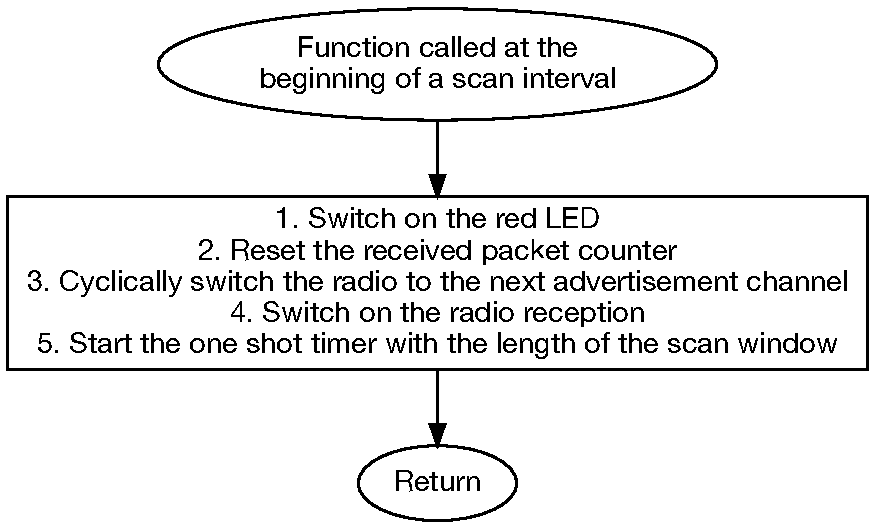
\includegraphics[scale=0.8]{scanInterval_chart}
\caption{Scan interval timer handler flowchart}
\label{fig:scanInterval_chart}
\end{figure}

\subsection{Scan Window Timer Handler}
The scan window timer is a single shot timer with an interval equal to the scan window. At the end of the scan window this function performs 3 different tasks as shown \ref{fig:scanWindow_chart}.
\begin{figure}[h]
\centering
\vspace{20pt}
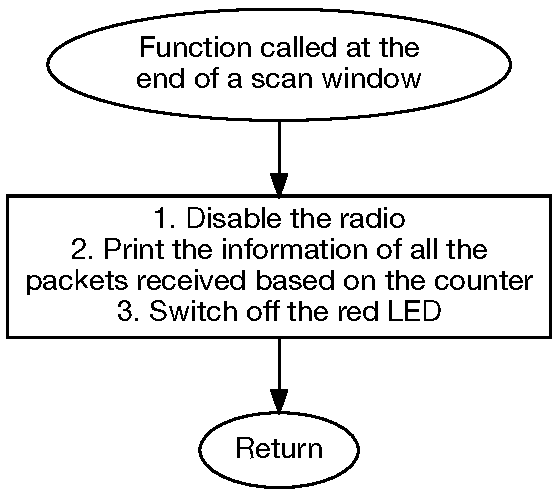
\includegraphics[scale=0.8]{scanWindow_chart}
\caption{Scan window timer handler flowchart}
\label{fig:scanWindow_chart}
\end{figure}
\clearpage

\subsection{Radio Interrupt Routine}
The radio peripheral is configured such that the end of a packet and the end of \acrshort{rssi} measurement trigger the interrupt. At the end of a packet, the packet's data is collected if there is space in the buffer. At the end of the \acrshort{rssi} measurement the \acrshort{rssi} value is saved. Note that when receiving a packet the `end of RSSI measurement' event happens before the `end of packet' event. 

\begin{figure}[h]
\centering
\vspace{-10pt}
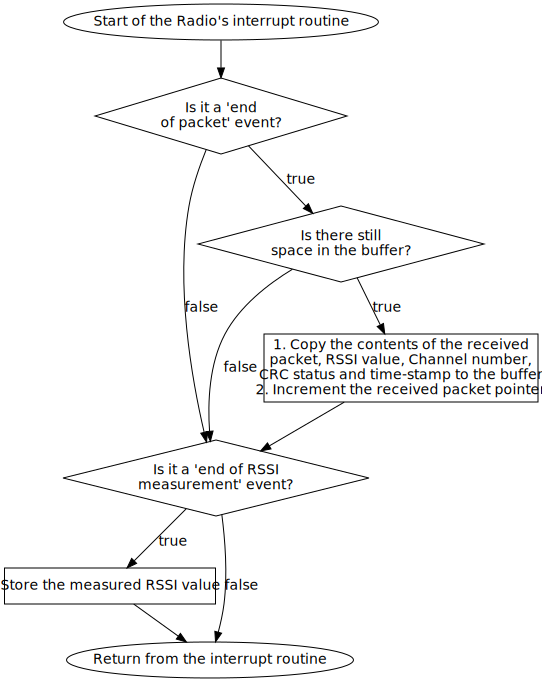
\includegraphics[scale=0.78]{RadioISR_chart}
\caption{Radio interrupt routine flowchart}
\label{fig:RadioISR_chart}
\vspace{-10pt}
\end{figure}

\chapter{Appendix | \texorpdfstring{\gls{ble}}{BLE} \texorpdfstring{\glspl{soc}}{SoCs} Comparison} \label{ApdxSoC}
The dense table in the next page compares many different parameters of the \gls{ble} \glspl{soc} available. This table was compiled in the first half of 2014. Because of the high pace at which the industry around \gls{ble} is progressing, many details here might not be accurate as time progresses.

The legend for the table is

\vspace{10pt}
NA \hspace{10pt}: The information is not available

- \hspace{22pt}: The feature is not available

\includepdf[pagecommand={\begin{tikzpicture} [remember picture,overlay] \node at (7.4,-17) {}; \end{tikzpicture}}]{BLE_SoCs.pdf}

\chapter{Data Acquired} \label{ApdxData}

The entire data acquired and results computed for both High-Throughput test and Request-Response test can be found in the tables in the following pages.

%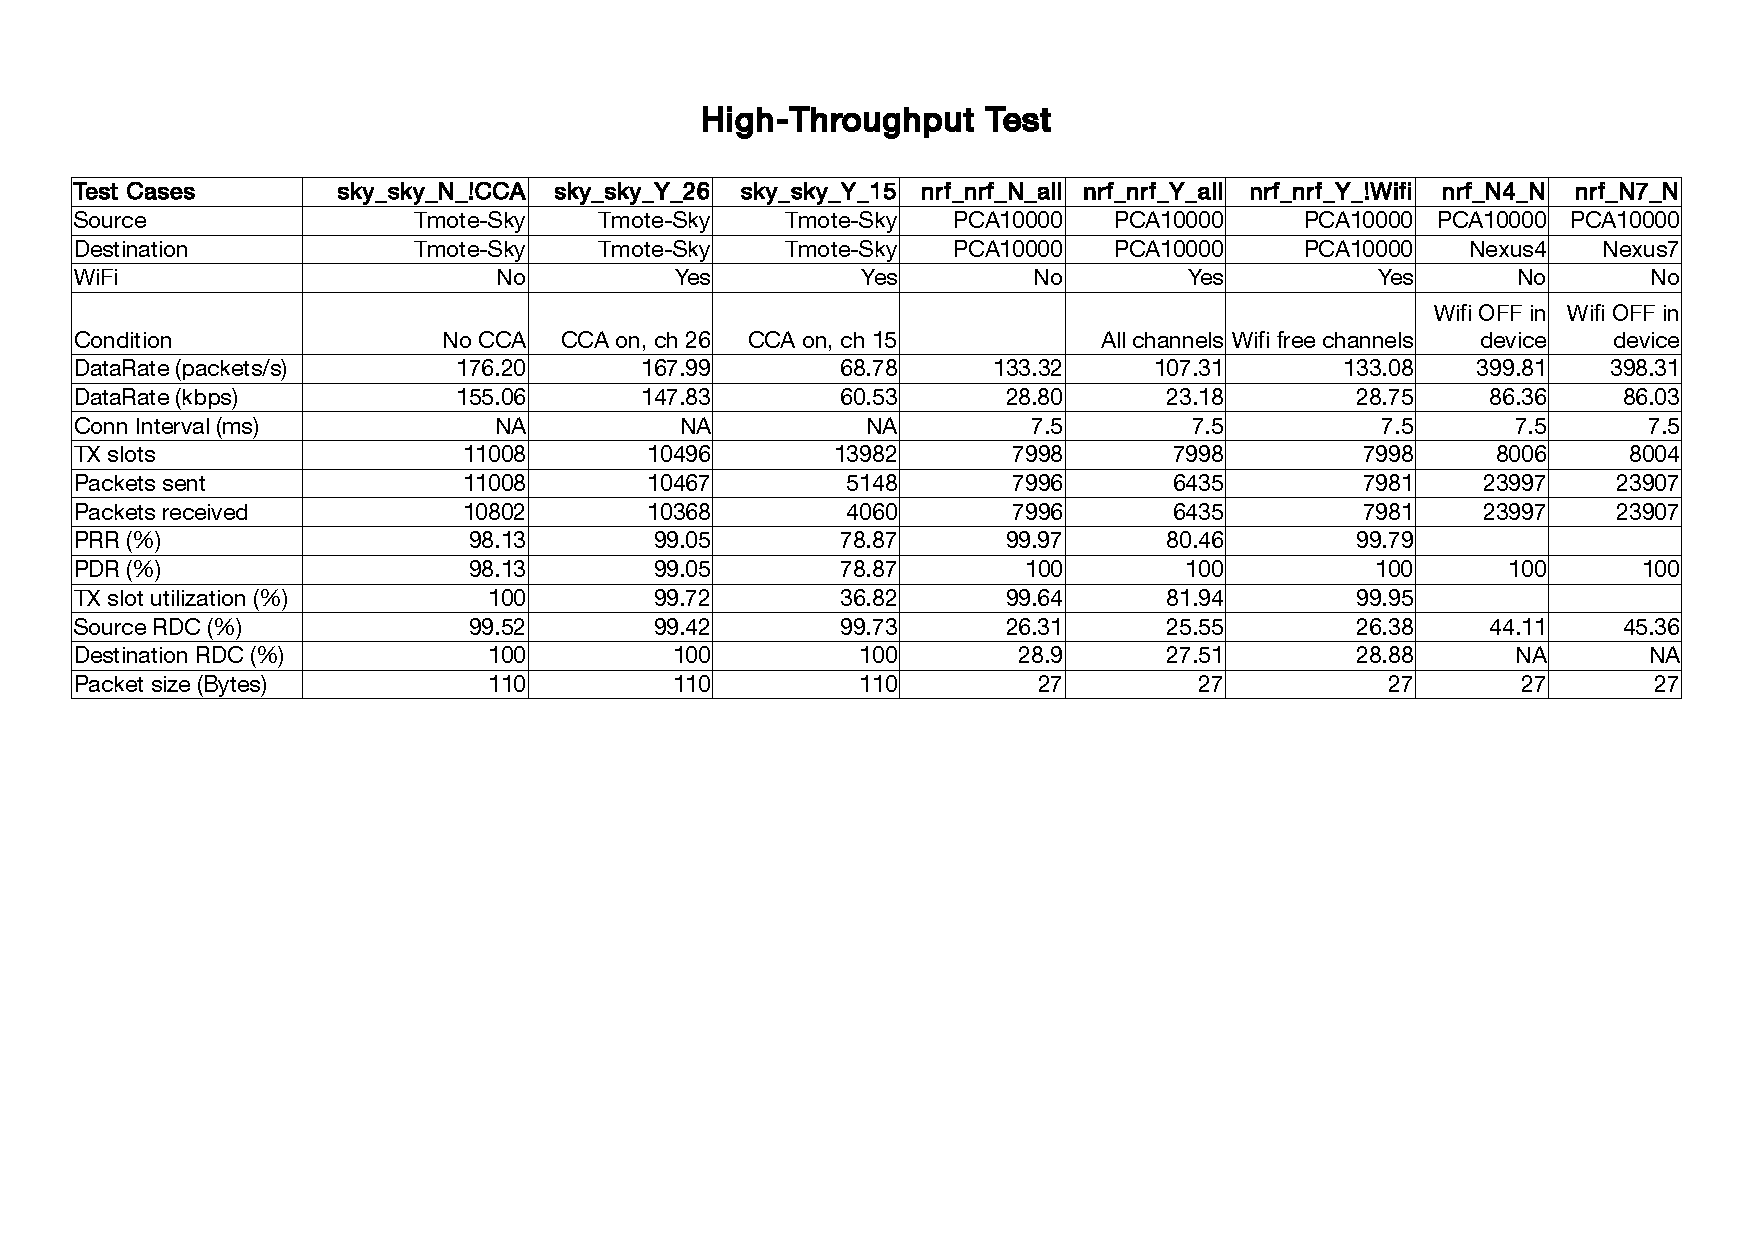
\includepdf[landscape]{HT.pdf}
%
%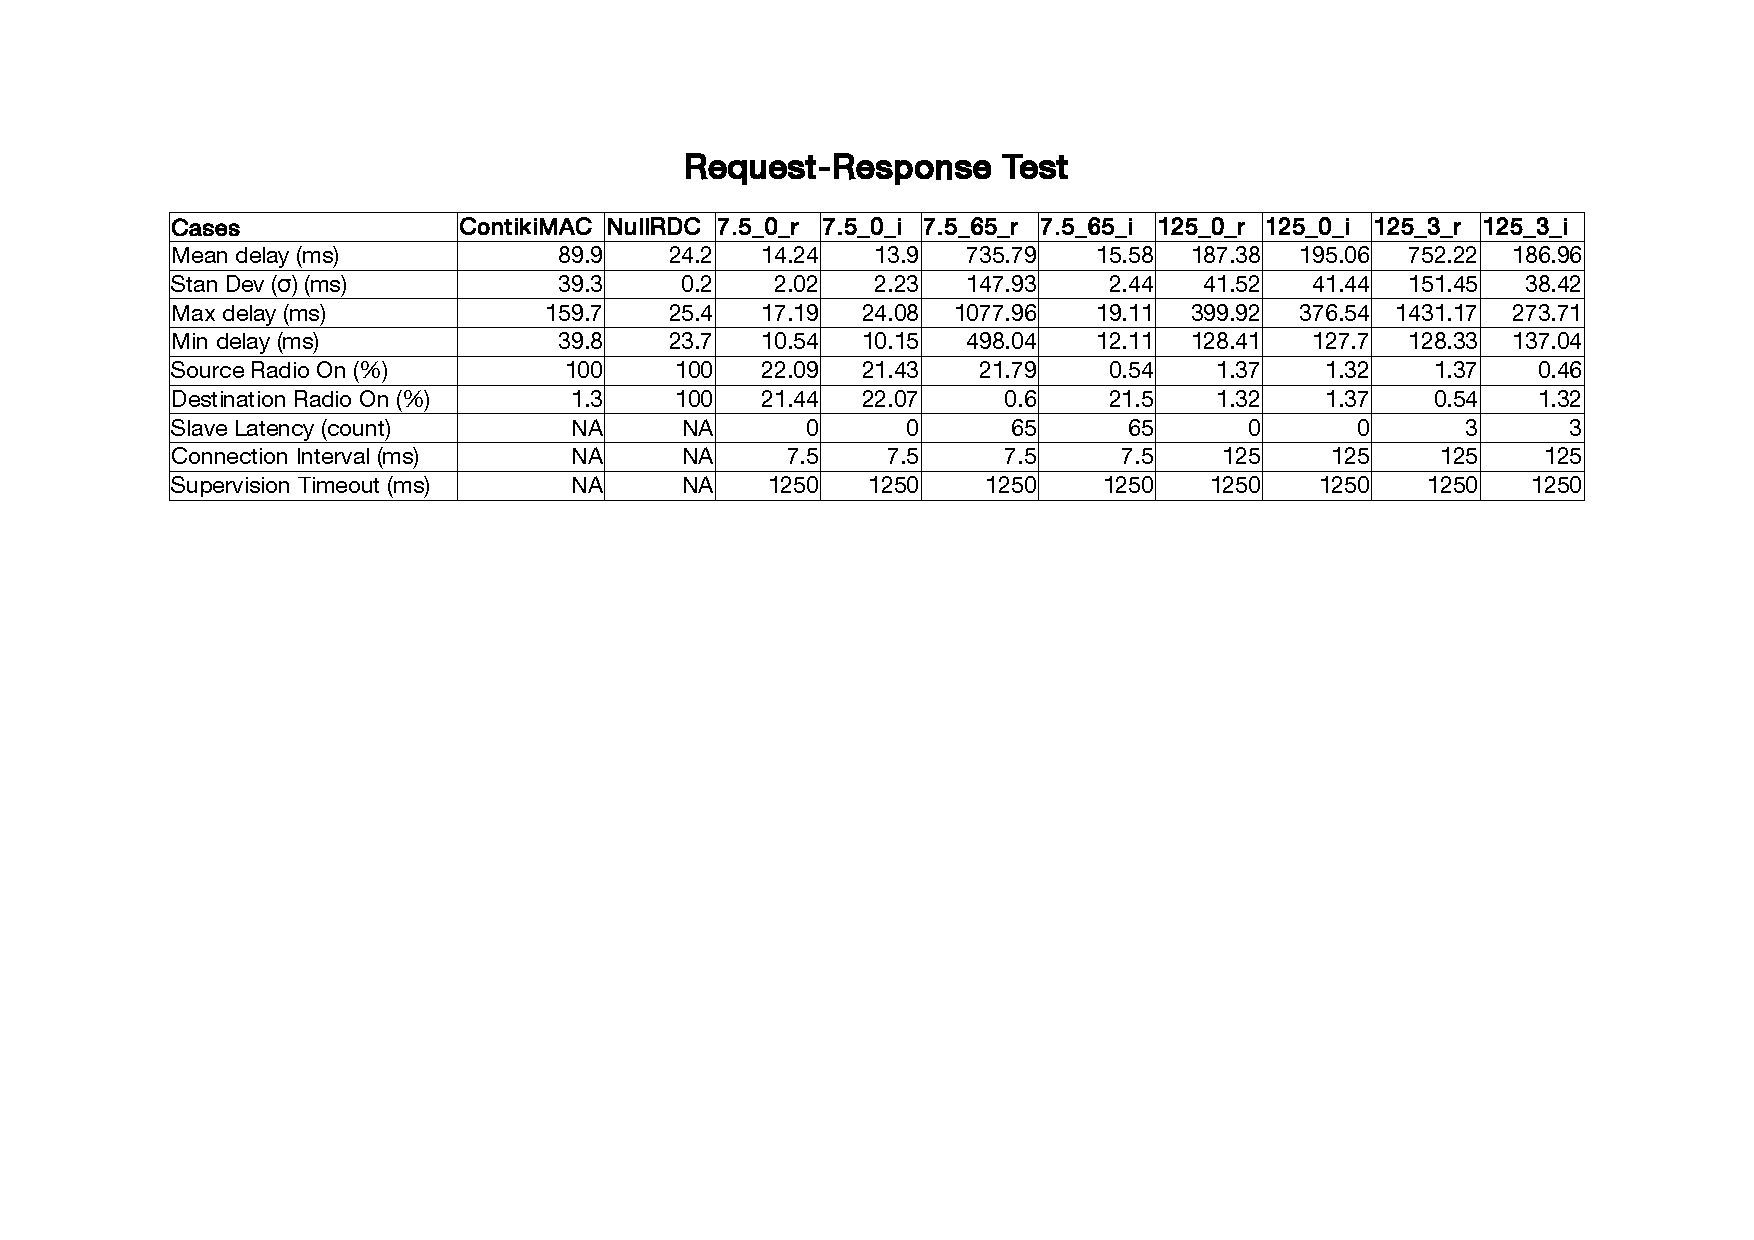
\includepdf[landscape]{RR.pdf}